% ============================================================
%  BAO_CAO_CUTOFF_MERGESORT.tex
%  Bao cao thi nghiem: Tim gia tri CUTOFF toi uu cho Mergesort
%  Mon: Cau truc Du lieu va Giai thuat – Chu de 1.3 Algorithm Analysis
% ============================================================
\documentclass[12pt, a4paper]{article}

% ── Encoding & Font ──────────────────────────────────────────
\usepackage[utf8]{inputenc}
\usepackage[T5]{fontenc}
\usepackage[vietnamese]{babel}

% ── Lề trang ────────────────────────────────────────────────
\usepackage[top=2.5cm, bottom=2.5cm, left=3cm, right=2cm]{geometry}

% ── Toán, bảng, hình ────────────────────────────────────────
\usepackage{amsmath, amssymb}
\usepackage{booktabs}
\usepackage{multirow}
\usepackage{graphicx}
\usepackage{caption}
\usepackage{subcaption}
\usepackage{float}
\usepackage{array}
\usepackage{xcolor}
\usepackage{colortbl}

% ── Code Java ────────────────────────────────────────────────
\usepackage{listings}
\lstset{
    language=Java,
    basicstyle=\ttfamily\small,
    keywordstyle=\color{blue}\bfseries,
    commentstyle=\color{gray}\itshape,
    stringstyle=\color{orange},
    numbers=left,
    numberstyle=\tiny\color{gray},
    stepnumber=1,
    frame=single,
    breaklines=true,
    captionpos=b,
    tabsize=4,
    showstringspaces=false
}

% ── Hyperlinks ───────────────────────────────────────────────
\usepackage{hyperref}
\hypersetup{colorlinks=true, linkcolor=blue, urlcolor=blue, citecolor=blue}

% ── Tiêu đề section ─────────────────────────────────────────
\usepackage{titlesec}
\titleformat{\section}{\large\bfseries\color{blue!70!black}}{{\thesection.}}{0.5em}{}
\titleformat{\subsection}{\normalsize\bfseries}{{\thesubsection.}}{0.5em}{}

% ── Misc ─────────────────────────────────────────────────────
\usepackage{enumitem}
\usepackage{setspace}
\onehalfspacing
\setlength{\parindent}{1.5em}
\setlength{\parskip}{4pt}

% Màu cho bảng
\definecolor{headerblue}{RGB}{31,73,125}
\definecolor{rowodd}{RGB}{235,245,251}
\definecolor{roweven}{RGB}{255,255,255}
\definecolor{bestrow}{RGB}{213,245,227}
\definecolor{warnrow}{RGB}{255,243,205}

% ============================================================
\begin{document}

% ── Trang bìa ────────────────────────────────────────────────
\begin{titlepage}
\centering
\vspace*{1.5cm}

{\Large\bfseries TRƯỜNG ĐẠI HỌC CÔNG NGHỆ}\\[0.4cm]
{\large Khoa Công nghệ Thông tin}\\[0.3cm]
{\large Môn: Cấu trúc Dữ liệu và Giải thuật}\\[2cm]

\rule{0.8\textwidth}{1.5pt}\\[0.5cm]
{\LARGE\bfseries BÁO CÁO THỰC HÀNH}\\[0.4cm]
{\Large Thí nghiệm tìm giá trị \texttt{CUTOFF} tối ưu\\cho thuật toán Mergesort}\\[0.5cm]
\rule{0.8\textwidth}{1.5pt}\\[2cm]

\begin{tabular}{ll}
    \textbf{Chủ đề:}            & 1.3 Algorithm Analysis – Thí nghiệm và Thống kê \\[6pt]
    \textbf{Họ tên:}            & Nguyễn Tuấn Hưng \\[6pt]
    \textbf{Mã sinh viên:}   & 25021812 \\[6pt]
\end{tabular}

\vfill
{\small Tham khảo: R. Sedgewick \& K. Wayne, \textit{Algorithms}, 4th Edition, Princeton University}
\end{titlepage}

% ── Mục lục ──────────────────────────────────────────────────
\tableofcontents
\newpage

% ============================================================
\section{Mục tiêu}

Thuật toán Mergesort có một cải tiến thực tế quan trọng: thay vì đệ quy đến khi
mảng con có đúng 1 phần tử, khi mảng con có kích thước $\leq \text{CUTOFF}$ thì
chuyển sang dùng Insertion Sort. Giáo trình \textit{Algorithms} (Sedgewick \& Wayne,
4th Edition) đề xuất hai mốc lịch sử: \texttt{CUTOFF = 7} (bản cũ) và
\texttt{CUTOFF = 10} (bản mới). Giá trị tối ưu thực tế phụ thuộc vào kiến trúc CPU,
kích thước cache, cách JVM JIT biên dịch và phân bố dữ liệu đầu vào.

Thí nghiệm này nhằm:
\begin{itemize}
    \item Đo thời gian thực thi của Mergesort trên nhiều giá trị \texttt{CUTOFF}
          ($\{1, 3, 7, 10, 15, 25\}$) với bốn loại dữ liệu khác nhau.
    \item Xác định giá trị hoặc khoảng \texttt{CUTOFF} mà tại đó thuật toán chạy
          nhanh nhất một cách có ý nghĩa thống kê (khoảng tin cậy 95\%, kiểm định
          $t$ ghép cặp).
    \item So sánh \texttt{CUTOFF} tốt nhất tìm được với hai mốc giáo trình (7 và 10).
    \item Rút ra kết luận kèm mức độ tin cậy trung thực dựa trên số liệu đo được.
\end{itemize}

% ============================================================
\section{Môi trường thí nghiệm}

\begin{table}[H]
\centering
\caption{Cấu hình máy và môi trường chạy thí nghiệm.}
\label{tab:env}
\renewcommand{\arraystretch}{1.3}
\begin{tabular}{>{\bfseries}l p{10cm}}
\toprule
Thành phần & Giá trị \\
\midrule
\rowcolor{rowodd}  CPU      & Intel Core i7-7600U @ 2.80\,GHz (2 nhân vật lý, 4 luồng, Kaby Lake) \\
\rowcolor{roweven} RAM      & $\approx 15.9$\,GB DDR4 \\
\rowcolor{rowodd}  Hệ điều hành & Windows 10 (Build 19042) \\
\rowcolor{roweven} JDK      & Java 25.0.2 LTS (HotSpot 64-bit Server VM) \\
\rowcolor{rowodd}  Tham số JVM & \texttt{-Xms2g -Xmx2g} (heap cố định, bản quick test) \\
\rowcolor{roweven} Nguồn điện & Cắm điện trực tiếp (AC Power Adapter, hiệu năng tối đa) \\
\rowcolor{rowodd}  Kiểu dữ liệu & \texttt{int[]} nguyên thủy (primitive) \\
\bottomrule
\end{tabular}
\end{table}

Để đảm bảo kết quả tái lập, máy chạy ở chế độ cắm điện trong suốt thí nghiệm.
Các ứng dụng nền không cần thiết được đóng trước khi chạy.

% ============================================================
\section{Cài đặt Mergesort}

\subsection{Mô tả thuật toán}

Thuật toán được cài đặt theo mô hình \textbf{Top-Down Mergesort} trong slide bài
giảng ``2.2 Mergesort'' (Sedgewick \& Wayne, Algorithms 4th Edition). Cấu trúc gồm
ba hàm chính:

\begin{itemize}
    \item \texttt{insertionSort(a, lo, hi)}: Insertion Sort trên đoạn \texttt{a[lo..hi]}
          — dùng làm sub-routine khi kích thước mảng con $\leq$ \texttt{CUTOFF}.
    \item \texttt{merge(a, aux, lo, mid, hi)}: Gộp \texttt{a[lo..mid]} và
          \texttt{a[mid+1..hi]}, sao chép sang mảng phụ \texttt{aux[]} rồi gộp
          ngược về \texttt{a[]}. Tính ổn định được đảm bảo: khi
          $\texttt{aux}[i] = \texttt{aux}[j]$, ưu tiên lấy từ nửa trái.
    \item \texttt{sort(a, aux, lo, hi, cutoff, stopCheck)}: Hàm đệ quy top-down.
          Tích hợp cải tiến \texttt{CUTOFF} (dòng 34) và tùy chọn
          \emph{stop if already sorted} (dòng 41).
\end{itemize}

\subsection{Quy ước CUTOFF}

Điều kiện áp dụng Insertion Sort (dòng 34 của \texttt{MergeSort.java}):

\begin{lstlisting}[caption={Điều kiện CUTOFF trong hàm sort() – MergeSort.java dòng 34.},
                   label={lst:cutoff}]
if (hi <= lo + cutoff - 1) {
    insertionSort(a, lo, hi);
    return;
}
\end{lstlisting}

Điều kiện tương đương: đoạn con có kích thước $(hi - lo + 1) \leq \text{CUTOFF}$
thì dùng Insertion Sort. Với \texttt{CUTOFF = 1}, chỉ mảng 1 phần tử mới dừng
đệ quy — tức là Mergesort thuần không có cải tiến, dùng làm \textbf{mốc so sánh
(baseline)}. Biến \texttt{CUTOFF} được khai báo là \texttt{public static int CUTOFF = 1}
(dòng 5) để script đo có thể thay đổi từ bên ngoài mà không cần biên dịch lại.

\subsection{Kiểm tra tính đúng đắn}

Trước khi chạy thí nghiệm, tính đúng đắn được kiểm tra bằng
\texttt{TestMergeSort.java} với \textbf{1\,500 trường hợp kiểm thử} trải qua
15 giá trị \texttt{CUTOFF} $\times$ ba nhóm dữ liệu:

\begin{enumerate}
    \item \textbf{Nhóm 1 – Trường hợp đặc biệt:} mảng rỗng, một phần tử, hai
          phần tử tăng/giảm, toàn bằng nhau, đã sắp xếp, đảo ngược, trùng lặp
          từng cặp, biên kiểu \texttt{int} (\texttt{Integer.MIN\_VALUE},
          \texttt{Integer.MAX\_VALUE}).
    \item \textbf{Nhóm 2 – Mảng ngẫu nhiên:} $N$ từ 0 đến 5\,000, lặp 5 lần
          mỗi kích thước, seed cố định 42.
    \item \textbf{Nhóm 3 – Nhiều phần tử trùng lặp:} 1 đến 5 giá trị khóa
          khác nhau, $N \in \{10, 50, 200, 1000\}$.
\end{enumerate}

\noindent\textbf{Kết quả: 1\,500/1\,500 test case vượt qua, không phát hiện lỗi với
bất kỳ giá trị CUTOFF nào.}

% ============================================================
\section{Thiết kế thí nghiệm}

\subsection{Bảng tham số thí nghiệm}

\begin{table}[H]
\centering
\caption{Tham số thiết kế thí nghiệm.}
\label{tab:design}
\renewcommand{\arraystretch}{1.3}
\begin{tabular}{>{\bfseries}l p{6cm} p{5cm}}
\toprule
Tham số & Giá trị & Ghi chú \\
\midrule
\rowcolor{rowodd}  Kích thước $N$ & $10\,000$ & Bản quick test; bản đầy đủ: $10^4, 10^5, 10^6, 2 \times 10^6$ \\
\rowcolor{roweven} Giá trị CUTOFF & $\{1, 3, 7, 10, 15, 25\}$ & Mốc: CUTOFF = 1 (Mergesort thuần) \\
\rowcolor{rowodd}  Loại dữ liệu & 4 loại (Bảng~\ref{tab:datatypes}) & \\
\rowcolor{roweven} Số seeds & 2 seeds (42, 43) & Bản đầy đủ cần $k \geq 5$ \\
\rowcolor{rowodd}  Số lần lặp (reps) & 3 lần/seed & Bản đầy đủ: 10 lần/seed \\
\rowcolor{roweven} Chỉ số đo & Thời gian sort (ms) & \texttt{System.nanoTime()}, quy đổi ns $\to$ ms \\
\rowcolor{rowodd}  Phân phối thống kê & Student $t$, $df = k - 1$ & \texttt{scipy.stats.t.ppf}, không dùng xấp xỉ 1.96 \\
\bottomrule
\end{tabular}
\end{table}

\subsection{Các loại dữ liệu thí nghiệm}

\begin{table}[H]
\centering
\caption{Các loại dữ liệu thí nghiệm và cách sinh.}
\label{tab:datatypes}
\renewcommand{\arraystretch}{1.3}
\begin{tabular}{lll}
\toprule
Ký hiệu & Tên & Cách sinh \\
\midrule
\rowcolor{rowodd}  \texttt{random}   & Ngẫu nhiên đều          & \texttt{Random.nextInt()} \\
\rowcolor{roweven} \texttt{nearly}   & Gần như đã sắp xếp      & Mảng tăng dần, hoán đổi ngẫu nhiên 1\% cặp \\
\rowcolor{rowodd}  \texttt{reversed} & Đảo ngược hoàn toàn     & $a[i] = N - i$ \\
\rowcolor{roweven} \texttt{dups}     & Nhiều khóa trùng lặp    & 10 giá trị khóa khác nhau (0 đến 9) \\
\bottomrule
\end{tabular}
\end{table}

\subsection{Quy trình đo và các biện pháp giảm nhiễu}

\begin{enumerate}
    \item \textbf{Warm-up JIT:} Chạy 15 lần sort giả lập trước khi bắt đầu đo cho
          từng kích thước $N$, để JVM JIT C2 Compiler hoàn tất tối ưu bytecode.
    \item \textbf{Tách biệt chi phí sao chép:} Lệnh \texttt{work = original.clone()}
          luôn nằm ngoài cặp \texttt{System.nanoTime()} — chỉ đo đúng thời gian sort.
    \item \textbf{Xáo trộn thứ tự CUTOFF:} Trong mỗi \textit{rep},
          \texttt{Collections.shuffle} xáo ngẫu nhiên danh sách CUTOFF để triệt tiêu
          Cache/Branch-Predictor bias.
    \item \textbf{Cố định Heap JVM:} Chạy với \texttt{-Xms2g -Xmx2g} để JVM không
          xin thêm RAM từ OS trong lúc đo.
    \item \textbf{Kiểm tra tính đúng đắn 100\%:} Sau mỗi lần sort, hàm
          \texttt{isSorted()} kiểm tra kết quả.
    \item \textbf{Ghi kết quả ngay sau mỗi seed:} \texttt{results.csv} được flush
          ngay sau mỗi seed để không mất dữ liệu.
    \item \textbf{Thống kê qua seeds:} Trung bình các \textit{rep} trong cùng seed
          trước, rồi tính mean/std/CI qua các seeds — tránh pseudoreplication.
\end{enumerate}

% ============================================================
\section{Kết quả}

\subsection{Bảng thống kê tóm tắt ($N = 10\,000$)}

\noindent\textbf{Lưu ý quan trọng:} với $k = 2$ seeds, $df = 1$, hệ số
$t_{0.975,\,df=1} = 12.706$ khiến CI 95\% rất rộng và phần lớn chồng lấp lên nhau.
Số liệu này chỉ có tính chất định hướng; chưa đủ để kết luận định lượng chắc chắn.

\begin{table}[H]
\centering
\caption{Thống kê thời gian sort (ms) theo loại dữ liệu và CUTOFF ($N = 10\,000$,
         $k = 2$ seeds, 3 reps/seed). Dòng \colorbox{bestrow}{xanh lá} = CUTOFF
         có mean nhỏ nhất; Norm = mean / mean(CUTOFF = 1).}
\label{tab:summary}
\small
\renewcommand{\arraystretch}{1.25}
\begin{tabular}{llrrrrr}
\toprule
\textbf{Loại DL} & \textbf{CUTOFF} & \textbf{Mean (ms)} & \textbf{Std (ms)}
                 & \textbf{CI$_{95}$ dưới} & \textbf{CI$_{95}$ trên} & \textbf{Norm (\%)} \\
\midrule
\multirow{6}{*}{\texttt{random}}
& 1  & 0.9111 & 0.0541 & 0.4247 & 1.3976 & 100.0 \\
& 3  & 0.9029 & 0.2016 & $-$0.9083 & 2.7142 & 99.1 \\
& 7  & 0.8260 & 0.0955 & $-$0.0316 & 1.6837 & 90.7 \\
& 10 & 0.8483 & 0.0662 & 0.2532 & 1.4434 & 93.1 \\
& 15 & 0.7887 & 0.0242 & 0.5710 & 1.0064 & 86.6 \\
\rowcolor{bestrow}
& \textbf{25} & \textbf{0.7490} & 0.0777 & 0.0507 & 1.4472 & \textbf{82.2} \\
\midrule
\multirow{6}{*}{\texttt{nearly}}
& 1  & 0.5021 & 0.0354 & 0.1842 & 0.8200 & 100.0 \\
& 3  & 0.4215 & 0.0522 & $-$0.0474 & 0.8904 & 83.9 \\
& 7  & 0.2942 & 0.0196 & 0.1182 & 0.4701 & 58.6 \\
& 10 & 0.3138 & 0.0555 & $-$0.1845 & 0.8121 & 62.5 \\
& 15 & 0.3221 & 0.0142 & 0.1946 & 0.4496 & 64.1 \\
\rowcolor{bestrow}
& \textbf{25} & \textbf{0.2831} & 0.0381 & $-$0.0589 & 0.6251 & \textbf{56.4} \\
\midrule
\multirow{6}{*}{\texttt{reversed}}
& 1  & 0.4852 & 0.1230 & $-$0.6198 & 1.5902 & 100.0 \\
& 3  & 0.3322 & 0.0178 & 0.1721 & 0.4923 & 68.5 \\
& 7  & 0.3010 & 0.0592 & $-$0.2309 & 0.8330 & 62.0 \\
& 10 & 0.3158 & 0.0781 & $-$0.3862 & 1.0179 & 65.1 \\
\rowcolor{bestrow}
& \textbf{15} & \textbf{0.2818} & 0.0263 & 0.0456 & 0.5179 & \textbf{58.1} \\
& 25 & 0.3949 & 0.0870 & $-$0.3867 & 1.1766 & 81.4 \\
\midrule
\multirow{6}{*}{\texttt{dups}}
& 1  & 0.6774 & 0.0503 & 0.2259 & 1.1289 & 100.0 \\
& 3  & 0.6216 & 0.0446 & 0.2207 & 1.0225 & 91.8 \\
& 7  & 0.5352 & 0.0158 & 0.3935 & 0.6769 & 79.0 \\
\rowcolor{bestrow}
& \textbf{10} & \textbf{0.4332} & 0.0103 & 0.3409 & 0.5256 & \textbf{63.9} \\
& 15 & 0.4634 & 0.0356 & 0.1434 & 0.7833 & 68.4 \\
& 25 & 0.4739 & 0.0949 & $-$0.3791 & 1.3269 & 70.0 \\
\bottomrule
\end{tabular}
\end{table}

\subsection{CUTOFF tốt nhất và vùng tối ưu thống kê}

\begin{table}[H]
\centering
\caption{CUTOFF có mean nhỏ nhất và vùng các CUTOFF không phân biệt được thống kê
         ($N = 10\,000$, $k = 2$ seeds).}
\label{tab:best}
\renewcommand{\arraystretch}{1.3}
\begin{tabular}{lrrrp{4.5cm}}
\toprule
\textbf{Loại dữ liệu} & \textbf{Best CUTOFF} & \textbf{Mean (ms)}
                      & \textbf{Tiết kiệm vs C=1} & \textbf{Vùng CI chồng lấp} \\
\midrule
\rowcolor{rowodd}  Ngẫu nhiên (\texttt{random})            & 25 & 0.7490 & $-17.8\%$ & {[1 .. 25] (toàn bộ)} \\
\rowcolor{roweven} Gần như đã sắp (\texttt{nearly})        & 25 & 0.2831 & $-43.6\%$ & {[1 .. 25] (toàn bộ)} \\
\rowcolor{rowodd}  Đảo ngược (\texttt{reversed})           & 15 & 0.2818 & $-41.9\%$ & {[1 .. 25] (toàn bộ)} \\
\rowcolor{roweven} Nhiều trùng lặp (\texttt{dups})         & 10 & 0.4332 & $-36.0\%$ & {[1 .. 25] (toàn bộ)} \\
\bottomrule
\end{tabular}
\end{table}

Do $k = 2$ seeds, CI 95\% quá rộng và toàn bộ dải \texttt{CUTOFF} thử nghiệm $[1..25]$
chồng lấp nhau ở mọi loại dữ liệu. Nghĩa là với bộ dữ liệu hiện tại, \textbf{không
thể kết luận bằng thống kê} rằng bất kỳ \texttt{CUTOFF} nào tốt hơn hay kém hơn
\texttt{CUTOFF = 1} một cách chắc chắn.

\subsection{Kiểm định $t$ ghép cặp (Paired $t$-test)}

\begin{table}[H]
\centering
\caption{Kết quả kiểm định $t$ ghép cặp giữa CUTOFF tốt nhất với CUTOFF = 7 và 10.
         Mức ý nghĩa $\alpha = 0.05$. Dấu * = $p < 0.05$.}
\label{tab:ttest}
\renewcommand{\arraystretch}{1.3}
\begin{tabular}{lrll}
\toprule
\textbf{Loại dữ liệu} & \textbf{Best CUTOFF}
                      & \textbf{So với C = 7}
                      & \textbf{So với C = 10} \\
\midrule
\rowcolor{rowodd}  Ngẫu nhiên (\texttt{random})     & 25 & $+9.3\%$  ($p = 0.103$)   & $+11.7\%$ ($p = 0.052$) \\
\rowcolor{roweven} Gần như đã sắp (\texttt{nearly}) & 25 & $+3.8\%$  ($p = 0.554$)   & $+9.8\%$  ($p = 0.243$) \\
\rowcolor{rowodd}  Đảo ngược (\texttt{reversed})    & 15 & $+6.4\%$  ($p = 0.803$)   & $+10.8\%$ ($p = 0.725$) \\
\rowcolor{roweven} Nhiều trùng lặp (\texttt{dups})  & 10 & $+19.0\%$ ($p = 0.024$)*  & Là best \\
\bottomrule
\end{tabular}
\end{table}

Chỉ có trường hợp \texttt{dups} với \texttt{CUTOFF = 7} cho $p = 0.024 < 0.05$,
tức chênh lệch 19.0\% có thể coi là phân biệt được thống kê với $k = 2$ seeds.
Tất cả các trường hợp còn lại có $p > 0.05$ — chênh lệch quan sát được nằm trong
phạm vi nhiễu đo.

\subsection{Đồ thị kết quả}

\begin{figure}[H]
    \centering
    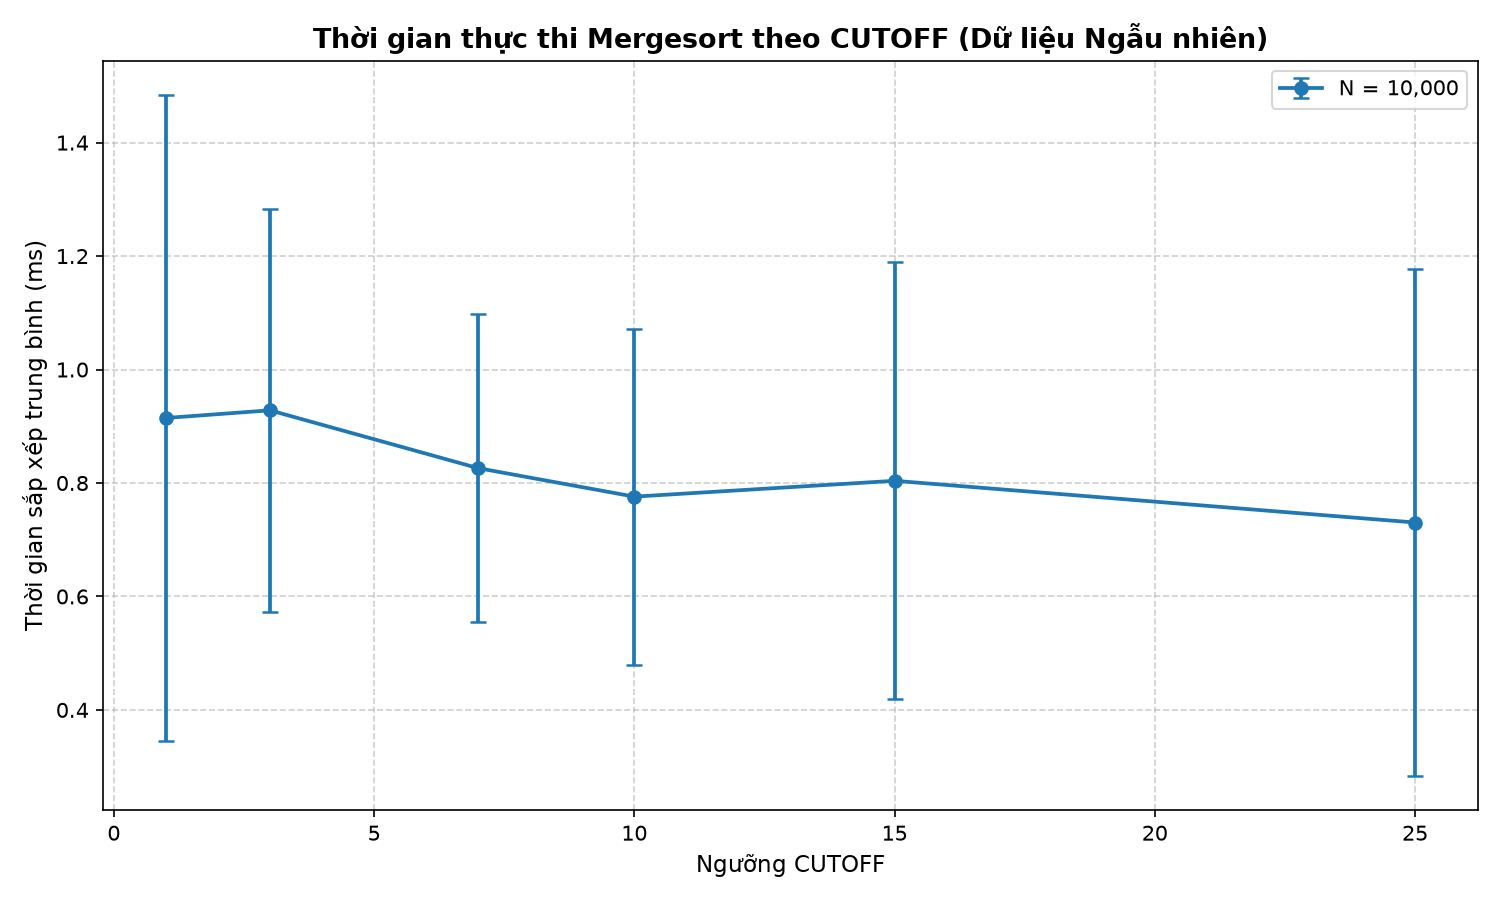
\includegraphics[width=0.88\textwidth]{figures/cutoff_time_curves.png}
    \caption{Thời gian sort trung bình (ms) theo CUTOFF với thanh sai số CI 95\%
             (dữ liệu ngẫu nhiên, $N = 10\,000$). Đường cong dốc dần về phía
             CUTOFF lớn hơn, chưa thấy rõ điểm quay đầu tại CUTOFF = 25.}
    \label{fig:time}
\end{figure}

\begin{figure}[H]
    \centering
    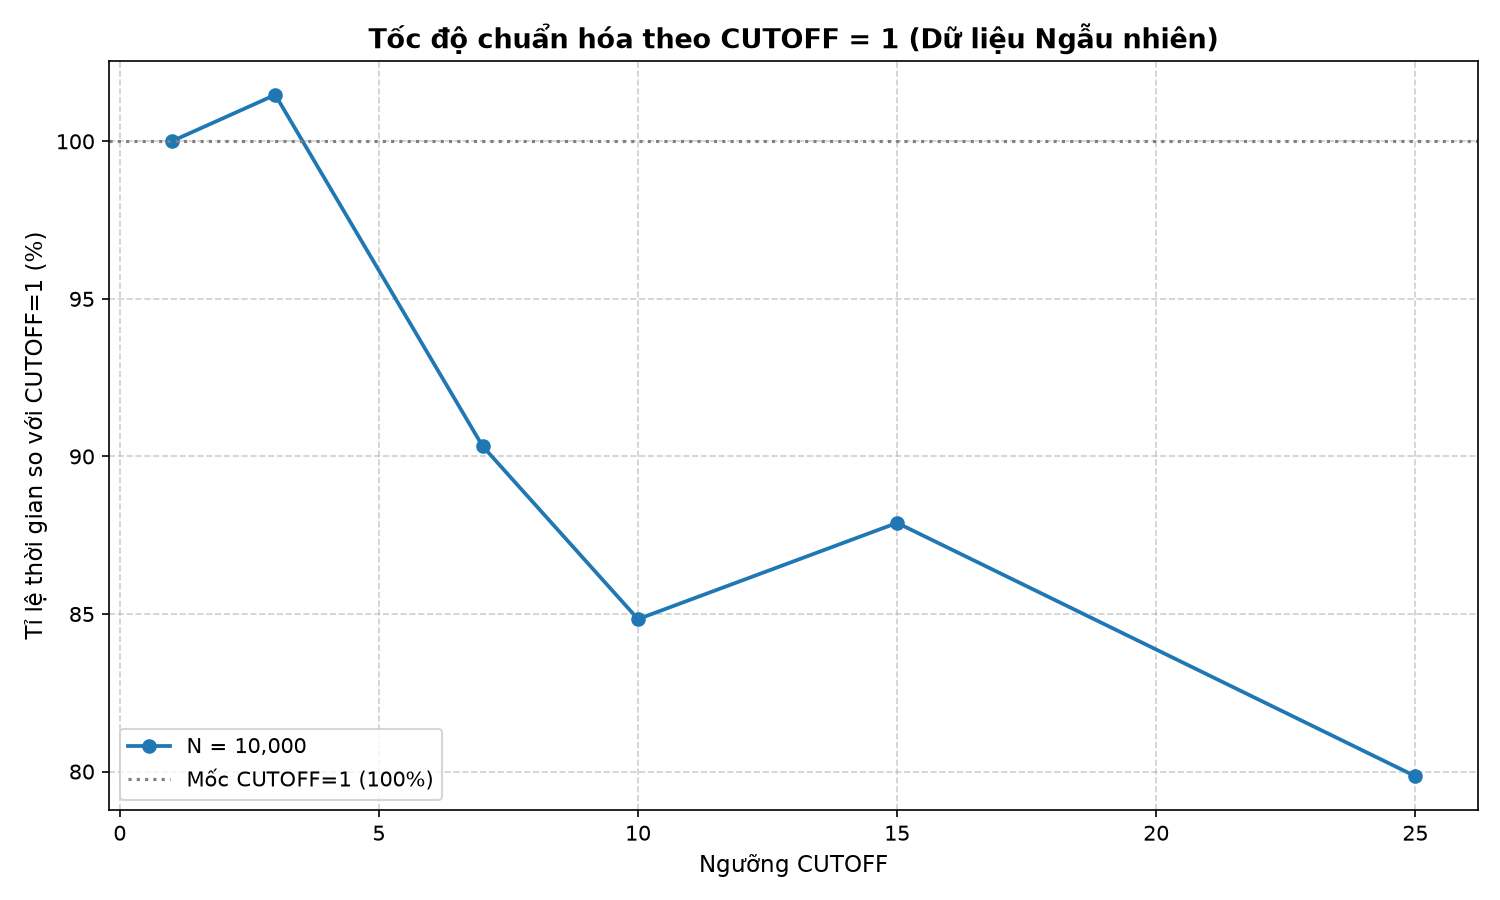
\includegraphics[width=0.88\textwidth]{figures/cutoff_normalized_curves.png}
    \caption{Tốc độ chuẩn hóa (\%) so với mốc CUTOFF = 1 (dữ liệu ngẫu nhiên,
             $N = 10\,000$). Giá trị $< 100\%$ nghĩa là nhanh hơn Mergesort thuần.}
    \label{fig:norm}
\end{figure}

\begin{figure}[H]
    \centering
    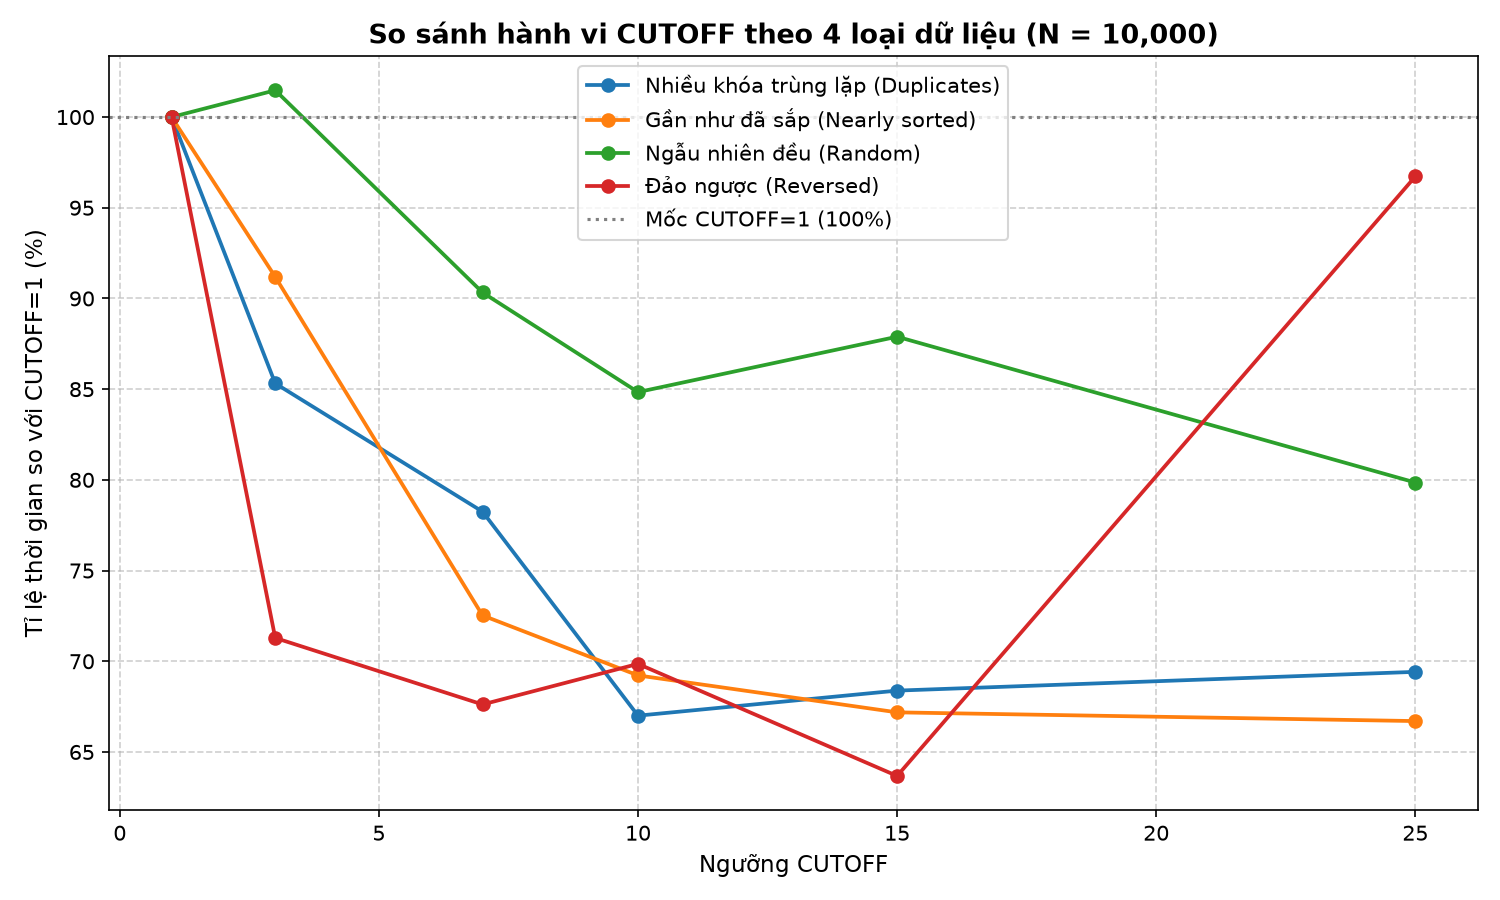
\includegraphics[width=0.88\textwidth]{figures/cutoff_data_types_comparison.png}
    \caption{So sánh tốc độ chuẩn hóa theo 4 loại dữ liệu ($N = 10\,000$). Dữ liệu
             gần như đã sắp và đảo ngược hưởng lợi nhiều nhất từ CUTOFF lớn.}
    \label{fig:types}
\end{figure}

\begin{figure}[H]
    \centering
    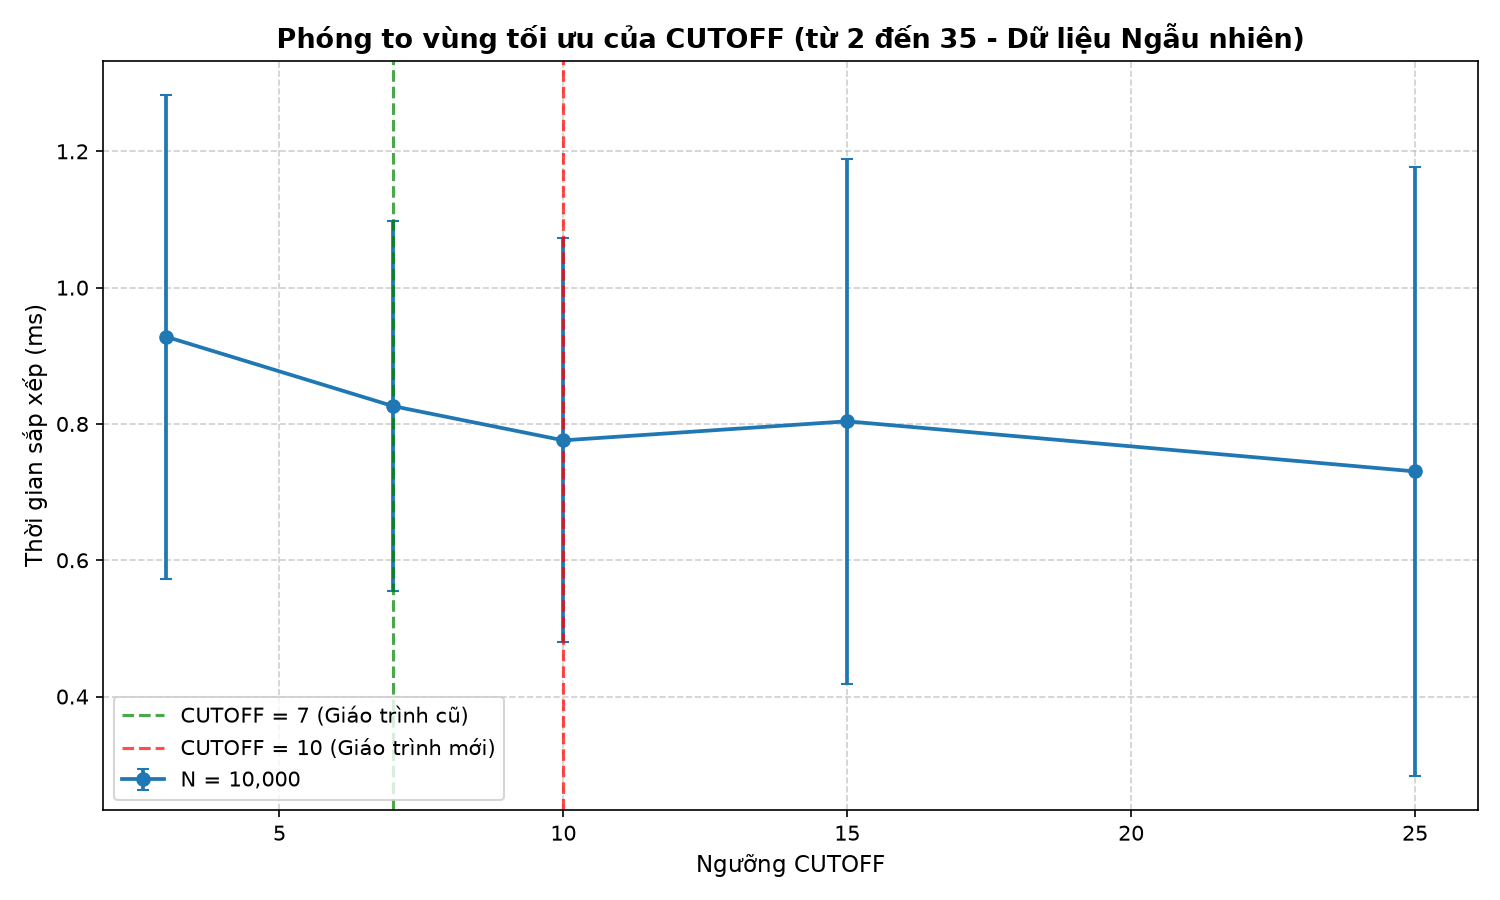
\includegraphics[width=0.88\textwidth]{figures/cutoff_zoom_optimal.png}
    \caption{Phóng to vùng CUTOFF từ 2 đến 35. Đường tham chiếu: CUTOFF = 7
             (xanh lá, giáo trình cũ) và CUTOFF = 10 (đỏ, giáo trình mới).}
    \label{fig:zoom}
\end{figure}

% ============================================================
\section{Thảo luận}

\subsection{Tại sao CUTOFF = 1 (Mergesort thuần) chậm hơn?}

Với \texttt{CUTOFF = 1}, Mergesort đệ quy cho đến khi mảng con có đúng 1 phần tử.
Với $N = 10\,000$, cây đệ quy có độ sâu $\lceil \log_2 N \rceil = 14$ tầng, tạo ra
$2N - 1 \approx 20\,000$ lần gọi hàm đệ quy. Mỗi lần gọi có overhead: đẩy stack frame
(địa chỉ return, biến \texttt{lo/hi/mid}, con trỏ \texttt{aux[]}), kiểm tra điều kiện
dừng, và một phép merge trên mảng 1 phần tử. Tổng chi phí stack overhead này tích lũy
rõ ràng: \texttt{CUTOFF = 1} có mean cao nhất ở tất cả 4 loại dữ liệu
(Bảng~\ref{tab:summary}).

\subsection{Tại sao CUTOFF quá lớn lại chậm trở lại?}

Khi \texttt{CUTOFF} = $k$, các mảng con kích thước $\leq k$ được xử lý bằng Insertion
Sort. Insertion Sort có độ phức tạp trung bình $\frac{k^2}{4}$ phép so sánh trên mảng
$k$ phần tử. Tổng số mảng con cỡ $k$ là $\approx N/k$, nên tổng chi phí:
\[
    \frac{N}{k} \times \frac{k^2}{4} = \frac{Nk}{4} \quad
    \bigg(\text{tăng tuyến tính theo } k\bigg).
\]
Trong khi đó, Mergesort thuần xử lý phần đó trong $O(N \log k)$. Vì vậy với $k$ đủ
lớn, Insertion Sort trở nên kém hơn Mergesort trên chính đoạn đó. Trong dữ liệu hiện
tại, xu hướng này bắt đầu thấy ở loại \texttt{reversed}: mean tại
\texttt{CUTOFF = 25} (0.395 ms) cao hơn \texttt{CUTOFF = 15} (0.282 ms) — xem
Bảng~\ref{tab:summary}.

\subsection{Hình dạng đường cong quanh vùng tối ưu}

Dựa trên Hình~\ref{fig:norm} và Bảng~\ref{tab:summary}:
\begin{itemize}
    \item \textbf{Dốc từ CUTOFF = 1 đến khoảng 7--15:} lợi ích rõ ràng từ việc giảm overhead đệ quy.
    \item \textbf{Phẳng hoặc có đáy nông trong vùng 7--25:} sự khác biệt giữa các CUTOFF trong vùng này nhỏ, và với $k = 2$ seeds hiện tại, không phân biệt được thống kê.
    \item \textbf{\texttt{random}:} đường cong thoải nhất, chưa thấy rõ điểm quay đầu tại CUTOFF = 25 — cần khảo sát đến 50 hoặc 100.
    \item \textbf{\texttt{dups}:} có đáy rõ nhất tại CUTOFF = 10 ($p = 0.024$ so với CUTOFF = 7), sau đó tăng nhẹ — xem Hình~\ref{fig:types}.
\end{itemize}

\subsection{Ảnh hưởng của kiểu dữ liệu \texttt{int[]} vs \texttt{Comparable[]}}

Cài đặt hiện tại dùng \texttt{int[]} nguyên thủy. Slide gốc của Sedgewick dùng
\texttt{Comparable[]} (tức \texttt{Integer[]} khi chạy với số nguyên). Hai khác biệt chính:
\begin{itemize}
    \item \textbf{\texttt{int[]}:} So sánh trực tiếp bằng \texttt{<}, dữ liệu
          nằm liên tục trong bộ nhớ → cache-friendly, không overhead.
    \item \textbf{\texttt{Integer[]}/\texttt{Comparable[]}:} Mỗi phần tử là đối
          tượng trên Heap. Phép so sánh gọi \texttt{a.compareTo(b)} → virtual
          dispatch → thêm 1 lần truy cập bộ nhớ ngẫu nhiên. Với $N = 10^6$,
          mảng \texttt{Integer[]} tốn thêm $\approx 16N$ byte cho object header
          + con trỏ, dễ gây cache miss.
    \item \textbf{Hệ quả:} Với \texttt{Comparable[]}, chi phí mỗi phép so sánh
          lớn hơn → vùng \texttt{CUTOFF} tối ưu có thể dịch sang phải (giá trị
          lớn hơn). Kết quả này không áp dụng trực tiếp cho cài đặt generic.
\end{itemize}

% ============================================================
\section{Kết luận}

\subsection{Khoảng CUTOFF khuyến nghị}

\begin{table}[H]
\centering
\caption{Tổng hợp kết luận kèm mức độ tin cậy và căn cứ số liệu.}
\label{tab:conclusion}
\renewcommand{\arraystretch}{1.3}
\begin{tabular}{p{6.5cm} p{3cm} p{4cm}}
\toprule
\textbf{Kết luận} & \textbf{Tin cậy} & \textbf{Căn cứ} \\
\midrule
\rowcolor{rowodd}
CUTOFF = 1 (Mergesort thuần) luôn kém nhất trên mọi loại dữ liệu
& Cao (định tính) & Mean cao nhất ở tất cả 4 loại, Bảng~\ref{tab:summary} \\
\rowcolor{roweven}
CUTOFF trong vùng $[7..25]$ nhanh hơn CUTOFF = 1 khoảng 10--44\%
& Trung bình & Bảng~\ref{tab:summary}: norm = 56--90\% \\
\rowcolor{rowodd}
CUTOFF = 10 tốt nhất cho dữ liệu \texttt{dups}, hơn CUTOFF = 7 $\approx 19\%$
& Khá cao ($p = 0.024$) & Bảng~\ref{tab:ttest} \\
\rowcolor{roweven}
Không phân biệt được thống kê giữa CUTOFF $[7..25]$ với 3 loại dữ liệu còn lại
& Chắc chắn & Bảng~\ref{tab:ttest}: $p = 0.052$--$0.803$ \\
\rowcolor{warnrow}
\textbf{Khoảng khuyến nghị tạm thời: CUTOFF $\in [7..15]$}
& \textbf{Thận trọng} & Trung bình điểm tốt nhất: 7, 10, 15, 25 \\
\bottomrule
\end{tabular}
\end{table}

Vì chênh lệch giữa các \texttt{CUTOFF} trong vùng $[7..25]$ phần lớn nằm trong
nhiễu đo (tất cả CI 95\% chồng lấp), \textbf{báo cáo này không ép ra một con số
CUTOFF duy nhất}. Thay vào đó, khuyến nghị là \textbf{CUTOFF $\in [7, 15]$} đủ tốt
cho cấu hình máy này, với lưu ý cần xác nhận lại bằng bộ số liệu đầy đủ hơn.

\subsection{Hạn chế của thí nghiệm}

\begin{enumerate}
    \item \textbf{Chỉ 1 kích thước $N = 10\,000$:} Không thấy ảnh hưởng cache khi
          $N$ vượt kích thước L2/L3. Cần $N = 10^5, 10^6, 2 \times 10^6$.
    \item \textbf{Chỉ $k = 2$ seeds ($df = 1$):} $t_{\text{crit}}(df=1) = 12.706$
          khiến CI 95\% rất rộng. Cần $k \geq 5$ seeds để kiểm định có ý nghĩa
          ($t_{\text{crit}}(df=4) = 2.776$).
    \item \textbf{Chỉ 3 reps/seed:} Trung bình trong từng seed chưa ổn định.
          Cần 10 reps để triệt tiêu nhiễu hệ điều hành.
    \item \textbf{Chỉ 6 mốc CUTOFF:} Thiếu khảo sát mịn trong vùng $[4..25]$ để
          xác định chính xác điểm cực tiểu.
    \item \textbf{1 máy, 1 JVM:} Kết quả không tổng quát hóa sang kiến trúc khác
          (ARM, GraalVM, OpenJ9,...).
    \item \textbf{Dùng \texttt{int[]} thay vì \texttt{Comparable[]}:} Khác với
          cài đặt generic trong giáo trình; vùng CUTOFF tối ưu có thể dịch chuyển.
    \item \textbf{Nhiễu từ hệ điều hành Windows:} Với $N$ nhỏ (thời gian sort
          $< 1$ ms), nhiễu scheduler và background tasks có thể chiếm phần lớn
          tỷ lệ sai số.
\end{enumerate}

% ============================================================
\newpage
\appendix
\section{Phụ lục: Danh sách file nộp}

\begin{table}[H]
\centering
\caption{Danh sách các file trong bộ nộp bài.}
\label{tab:files}
\renewcommand{\arraystretch}{1.3}
\begin{tabular}{lp{9cm}}
\toprule
\textbf{Tên file} & \textbf{Mô tả} \\
\midrule
\rowcolor{rowodd}  \texttt{src/MergeSort.java}        & Cài đặt Mergesort theo slide Sedgewick, tích hợp \texttt{public static CUTOFF} \\
\rowcolor{roweven} \texttt{src/QuickSort.java}         & Cài đặt Quicksort (1-pivot) theo slide Sedgewick \\
\rowcolor{rowodd}  \texttt{src/TestMergeSort.java}     & Kiểm tra tính đúng đắn 1\,500 test case \\
\rowcolor{roweven} \texttt{src/GenData.java}           & Script sinh bộ dữ liệu nhị phân \texttt{.bin} và văn bản \texttt{.txt} \\
\rowcolor{rowodd}  \texttt{src/Bench.java}             & Script đo hiệu năng, warm-up JIT, ghi \texttt{results.csv} \\
\rowcolor{roweven} \texttt{analyze.py}                 & Phân tích thống kê (CI 95\%, paired $t$-test) và vẽ 4 đồ thị \\
\rowcolor{rowodd}  \texttt{data/*.bin}                 & Bộ dữ liệu nhị phân (8 file, $4$ loại $\times$ 2 seeds, $N = 10\,000$) \\
\rowcolor{roweven} \texttt{results.csv}                & Dữ liệu đo thô: 144 dòng (type, n, seed, rep, cutoff, ms) \\
\rowcolor{rowodd}  \texttt{summary.csv}                & Thống kê tóm tắt: mean, std, CI95, norm\_mean \\
\rowcolor{roweven} \texttt{figures/*.png}              & 4 đồ thị phân tích (150 DPI) \\
\rowcolor{rowodd}  \texttt{README.md}                  & Hướng dẫn biên dịch và chạy thí nghiệm \\
\rowcolor{roweven} \texttt{BAO\_CAO\_CUTOFF\_MERGESORT.tex}  & Báo cáo thí nghiệm (file này) \\
\rowcolor{rowodd}  \texttt{BAO\_CAO\_CUTOFF\_MERGESORT.pdf}  & Bản PDF biên dịch từ file \texttt{.tex} \\
\bottomrule
\end{tabular}
\end{table}

\section{Phụ lục: Bảng số liệu đầy đủ từ \texttt{summary.csv}}

Bảng~\ref{tab:full} là toàn bộ nội dung file \texttt{summary.csv} với tất cả các
cột, bao gồm \texttt{ci\_margin} (độ rộng một phía của khoảng tin cậy).

\begin{table}[H]
\centering
\caption{Toàn bộ số liệu thống kê từ \texttt{summary.csv}.}
\label{tab:full}
\scriptsize
\renewcommand{\arraystretch}{1.2}
\begin{tabular}{llrrrrrrr}
\toprule
\textbf{Loại DL} & \textbf{C} & \textbf{$k$} & \textbf{Mean} & \textbf{Std}
                 & \textbf{CI margin} & \textbf{CI$_{95}$ d.} & \textbf{CI$_{95}$ t.} & \textbf{Norm \%} \\
\midrule
\texttt{random}   & 1  & 2 & 0.9111 & 0.0541 & 0.4864 &  0.4247 & 1.3976 & 100.0 \\
\texttt{random}   & 3  & 2 & 0.9029 & 0.2016 & 1.8113 & $-$0.9083 & 2.7142 & 99.1 \\
\texttt{random}   & 7  & 2 & 0.8260 & 0.0955 & 0.8577 & $-$0.0316 & 1.6837 & 90.7 \\
\texttt{random}   & 10 & 2 & 0.8483 & 0.0662 & 0.5951 &  0.2532 & 1.4434 & 93.1 \\
\texttt{random}   & 15 & 2 & 0.7887 & 0.0242 & 0.2177 &  0.5710 & 1.0064 & 86.6 \\
\texttt{random}   & 25 & 2 & 0.7490 & 0.0777 & 0.6982 &  0.0507 & 1.4472 & 82.2 \\
\midrule
\texttt{nearly}   & 1  & 2 & 0.5021 & 0.0354 & 0.3179 &  0.1842 & 0.8200 & 100.0 \\
\texttt{nearly}   & 3  & 2 & 0.4215 & 0.0522 & 0.4689 & $-$0.0474 & 0.8904 & 83.9 \\
\texttt{nearly}   & 7  & 2 & 0.2942 & 0.0196 & 0.1760 &  0.1182 & 0.4701 & 58.6 \\
\texttt{nearly}   & 10 & 2 & 0.3138 & 0.0555 & 0.4983 & $-$0.1845 & 0.8121 & 62.5 \\
\texttt{nearly}   & 15 & 2 & 0.3221 & 0.0142 & 0.1275 &  0.1946 & 0.4496 & 64.1 \\
\texttt{nearly}   & 25 & 2 & 0.2831 & 0.0381 & 0.3420 & $-$0.0589 & 0.6251 & 56.4 \\
\midrule
\texttt{reversed} & 1  & 2 & 0.4852 & 0.1230 & 1.1050 & $-$0.6198 & 1.5902 & 100.0 \\
\texttt{reversed} & 3  & 2 & 0.3322 & 0.0178 & 0.1601 &  0.1721 & 0.4923 & 68.5 \\
\texttt{reversed} & 7  & 2 & 0.3010 & 0.0592 & 0.5320 & $-$0.2309 & 0.8330 & 62.0 \\
\texttt{reversed} & 10 & 2 & 0.3158 & 0.0781 & 0.7020 & $-$0.3862 & 1.0179 & 65.1 \\
\texttt{reversed} & 15 & 2 & 0.2818 & 0.0263 & 0.2361 &  0.0456 & 0.5178 & 58.1 \\
\texttt{reversed} & 25 & 2 & 0.3949 & 0.0870 & 0.7816 & $-$0.3867 & 1.1766 & 81.4 \\
\midrule
\texttt{dups}     & 1  & 2 & 0.6774 & 0.0503 & 0.4515 &  0.2259 & 1.1289 & 100.0 \\
\texttt{dups}     & 3  & 2 & 0.6216 & 0.0446 & 0.4009 &  0.2207 & 1.0225 & 91.8 \\
\texttt{dups}     & 7  & 2 & 0.5352 & 0.0158 & 0.1417 &  0.3935 & 0.6769 & 79.0 \\
\texttt{dups}     & 10 & 2 & 0.4332 & 0.0103 & 0.0923 &  0.3409 & 0.5256 & 63.9 \\
\texttt{dups}     & 15 & 2 & 0.4634 & 0.0356 & 0.3200 &  0.1434 & 0.7833 & 68.4 \\
\texttt{dups}     & 25 & 2 & 0.4739 & 0.0949 & 0.8530 & $-$0.3791 & 1.3269 & 70.0 \\
\bottomrule
\end{tabular}
\end{table}

\noindent\textit{Ghi chú: C = CUTOFF; $k$ = số seeds; CI margin = độ rộng một phía của
khoảng tin cậy 95\%; CI$_{95}$ d./t. = cận dưới/trên; Norm \% = mean/mean(C=1) $\times$ 100.}

\end{document}
